\textbf{\underline{\large{1.6: Local Linearity, Euler's Method, and Approximations}}} \par

Before calculators, one of the most valuable uses of the derivative was to find approximate function values from a tangent line. Since the tangent line only shares one point on the function, $y$ values on the line are very close to $y$ values on the function. This idea is called local linearity—near the point of tangency, the function curve appears to be a line. This can be easily demonstrated with the graphing calculator by zooming in on the point of tangency. \par 

Consider the graphs of $y = \dfrac{1}{4}x^4$ and its tangent line at $x = 1$, given by the equation $y = x - \dfrac{3}{4}$: \par

\begin{center}
    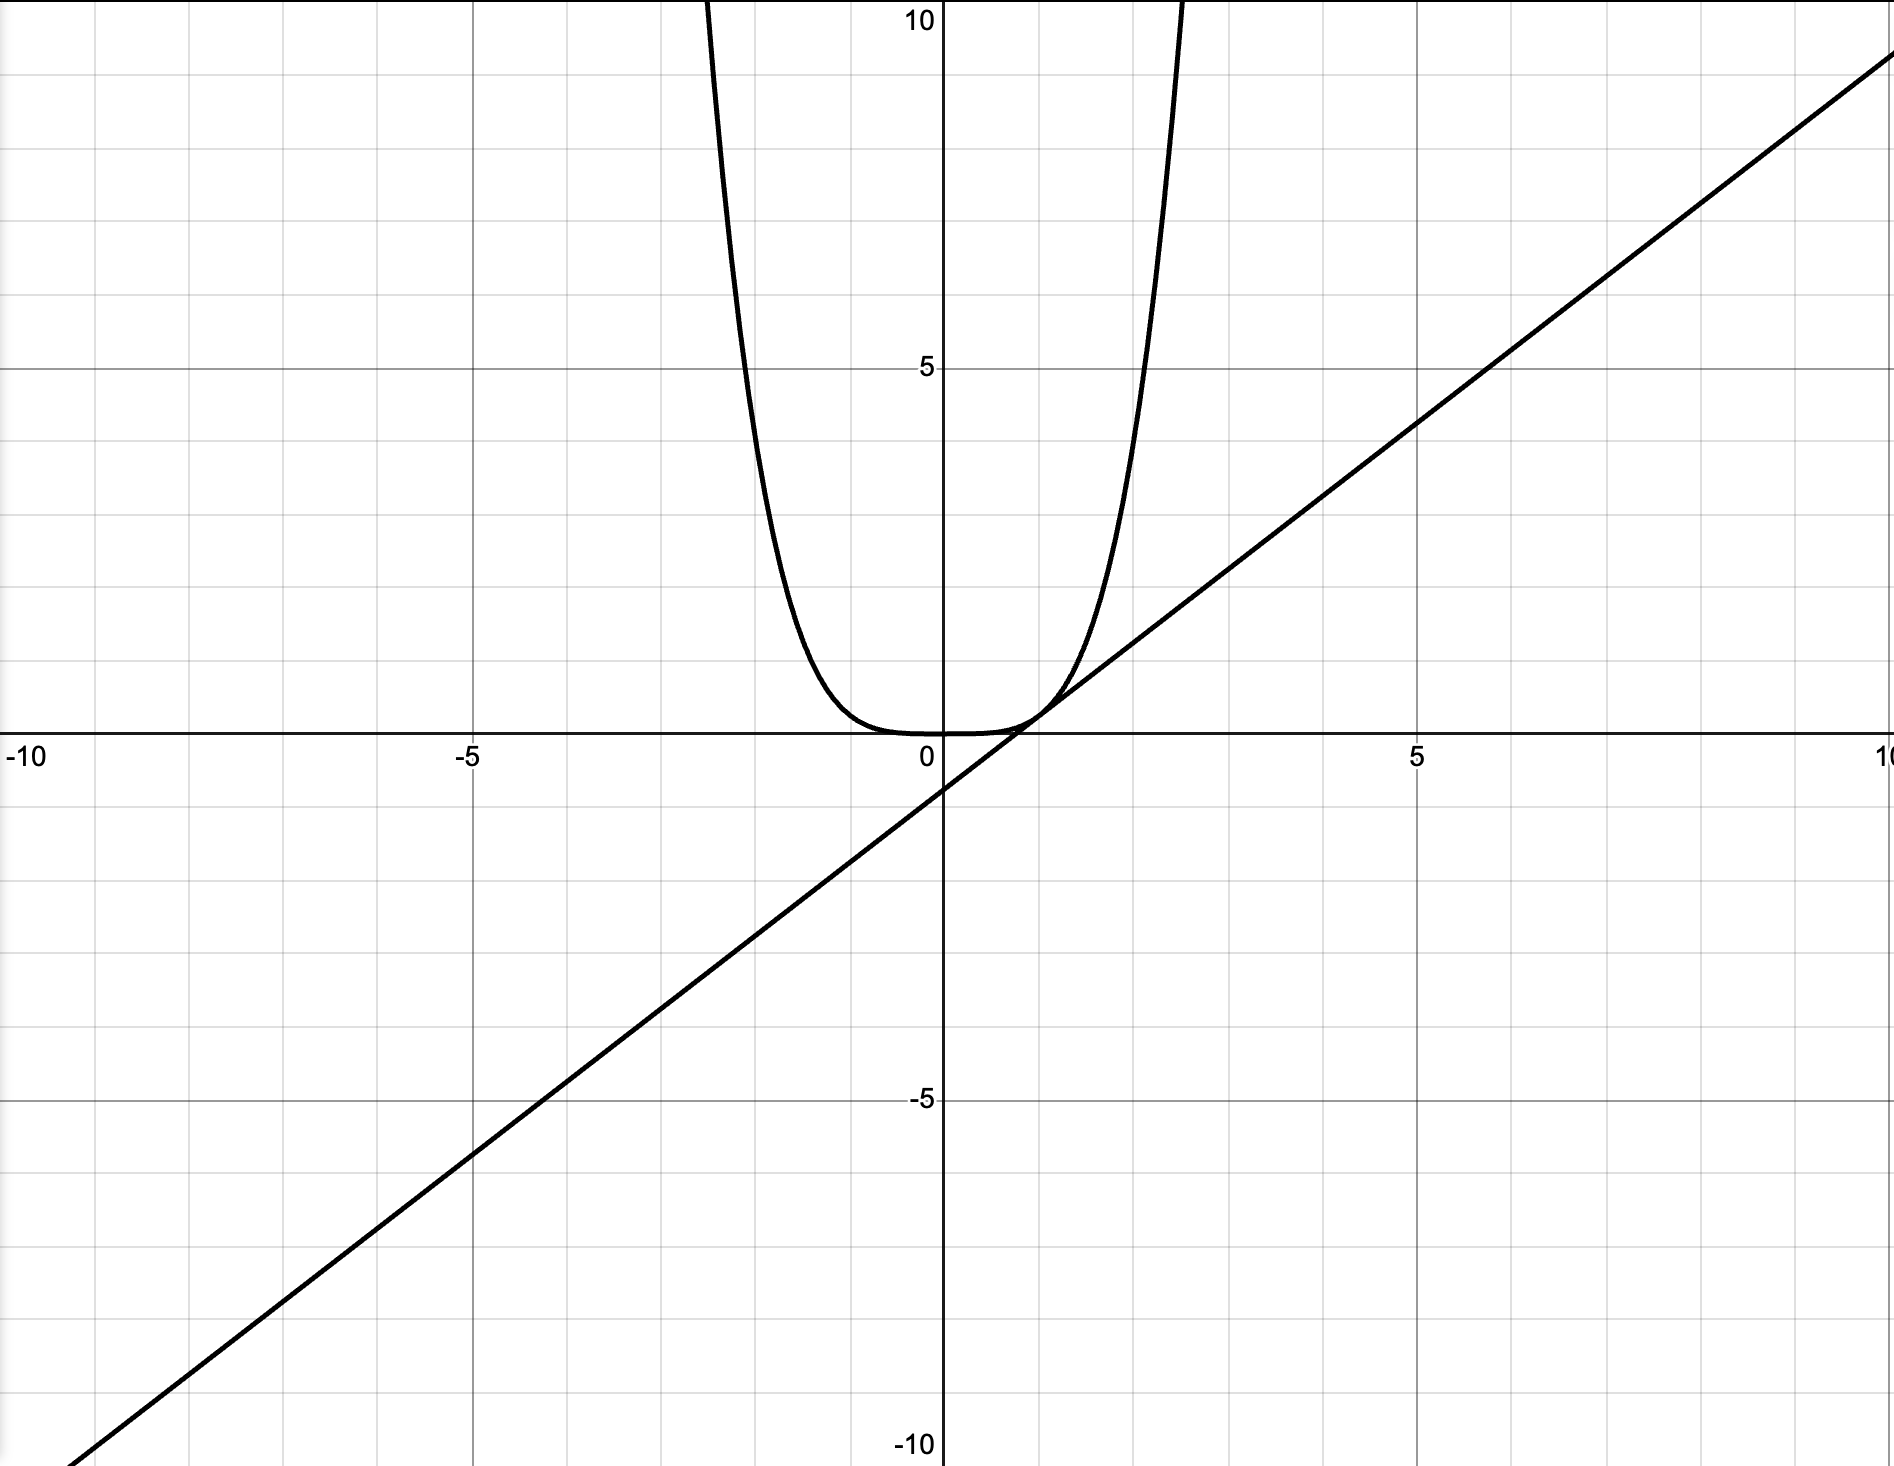
\includegraphics[width=0.49\textwidth]{Support/Chapter 1 Graphics/1.6-Graphic1.png}
    \hfill
    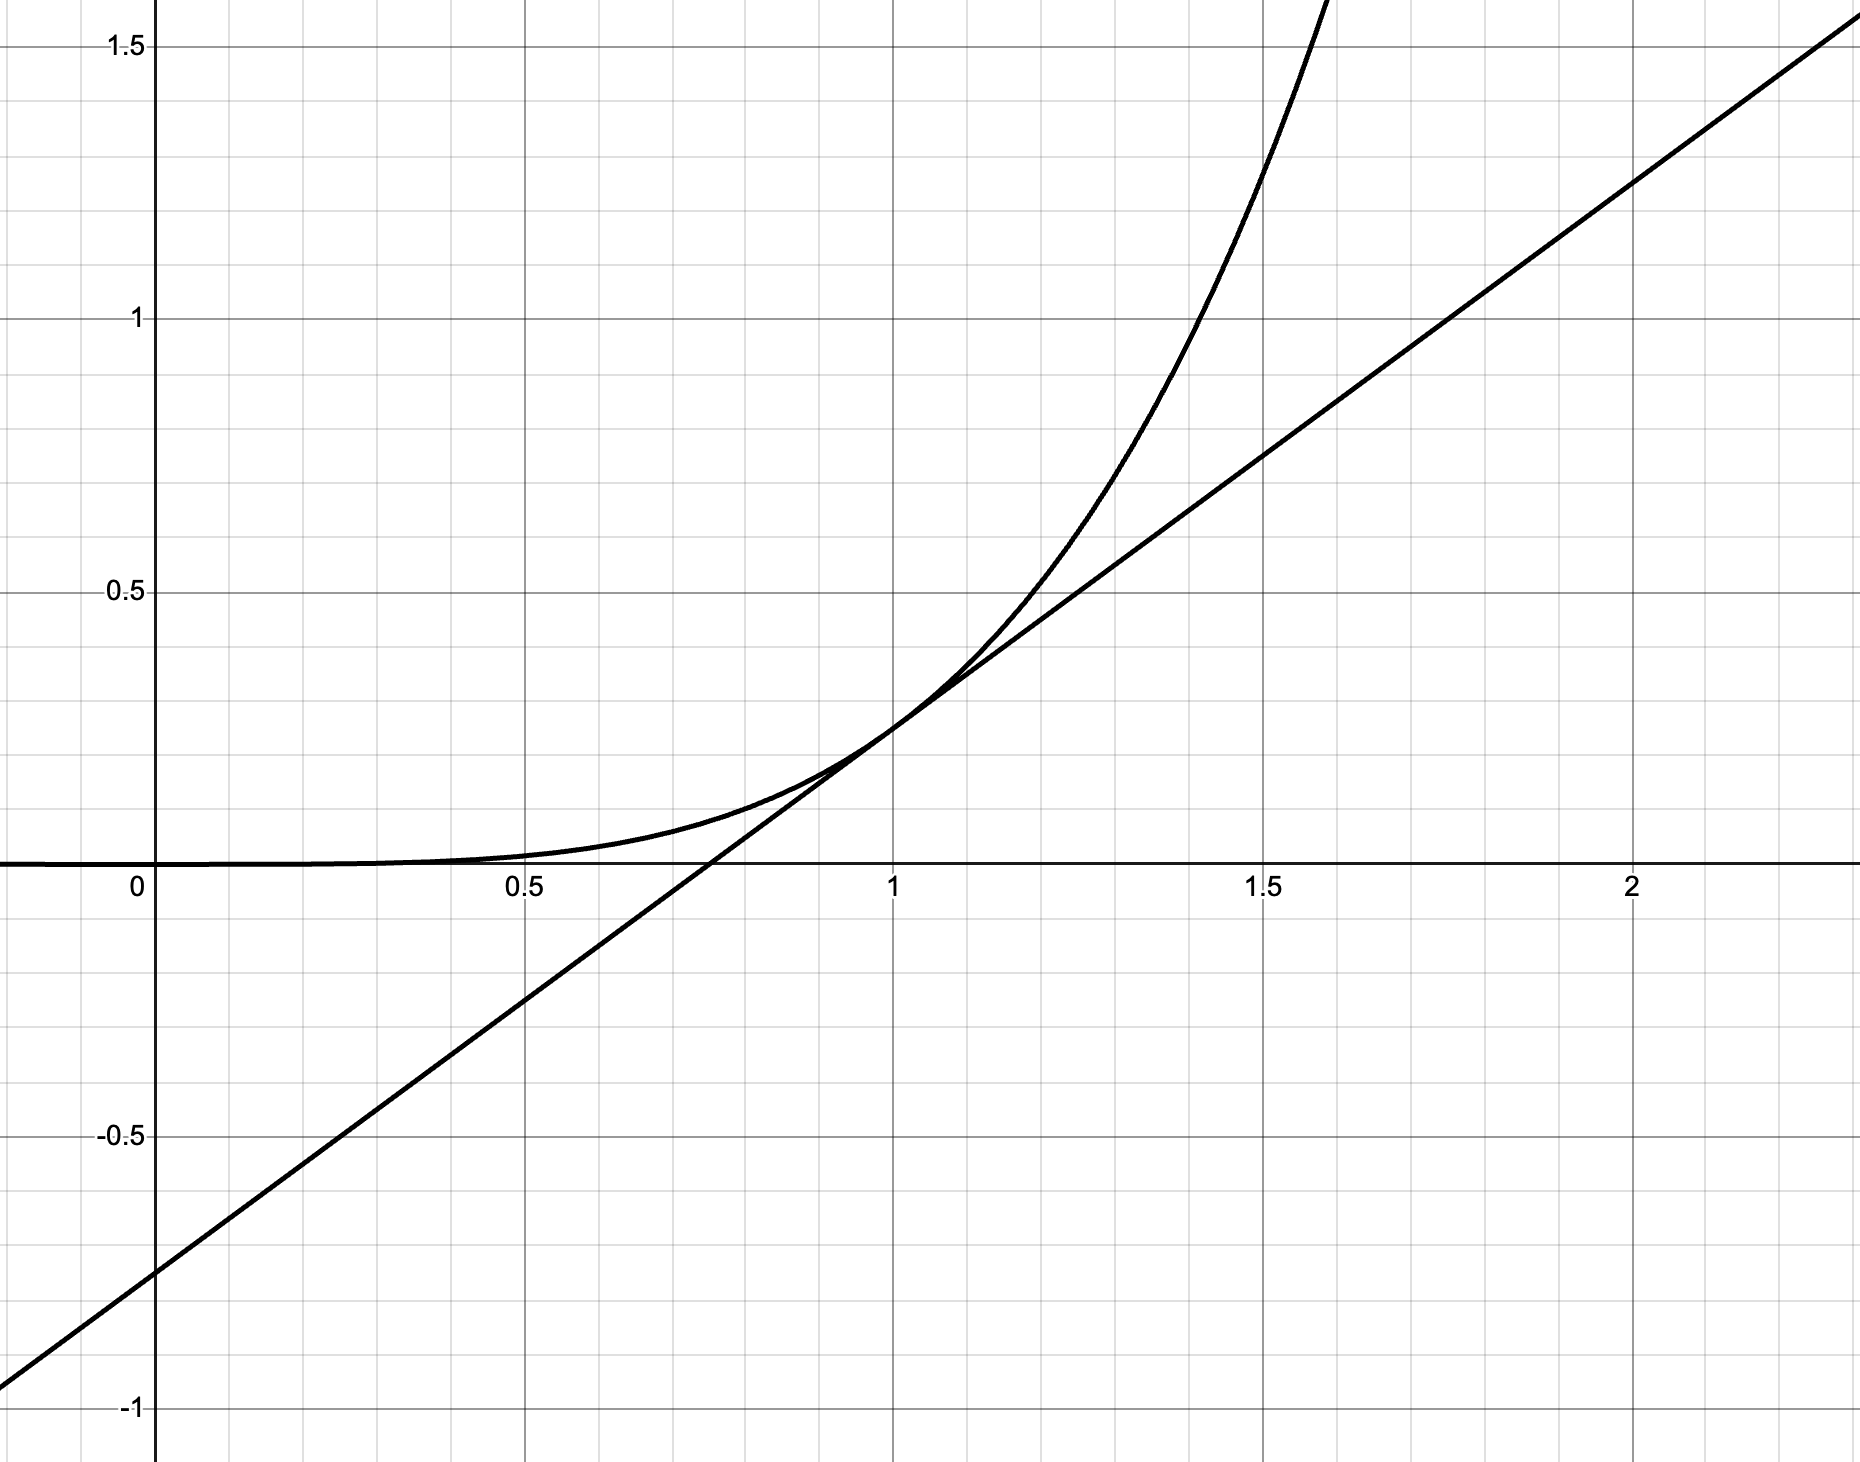
\includegraphics[width=0.49\textwidth]{Support/Chapter 1 Graphics/1.6-Graphic2.png}
\end{center}

The closer you zoom in, the more the line and the curve become one. The $y$ values on the line are good approximations of the $y$ values on the curve. For a good animation of this concept, see the following: \begin{align*}
    \href{https://drive.google.com/file/d/1lVYbRbXydqBz8KJWOfwWGO_c_oe58bC6/view?usp=sharing}{\text{\textcolor{blue}{tangent line approximation animation}}}
\end{align*} 

Since it's easier to find the $y$ value of a line arithmetically than for other functions --- especially transcendental functions --- the tangent line approximation is useful if you have no calculator. \par

\begin{tcolorbox}[objective]
    \begin{center}
        OBJECTIVES \\[11pt]
    \end{center}
    Use the Equation of a Tangent Line to Approximate Function Values.
\end{tcolorbox} \vspace{11pt}

\begin{tcolorbox}[example]
    \textbf{Ex 1.6.1: } Find the equations of the line tangent to $f(x) = x^4 - x^3 - 2x^2 + 1$ at $x = -1$. 
\end{tcolorbox}
\begin{tcolorbox}[solution]
    \textbf{Sol 1.6.1: } The slope of the tangent line will be $f'(-1)$ \begin{align*}
        & f'(x) = 4x^3 - 3x^2 - 4x \\[11pt]
        & f'(-1) = 4(-1)^3 - 3(-1)^2 - 4(-1) = -3 
    \end{align*} 
    (Note that we could've gotten this more easily with the nDeriv function on our calculator.) \begin{align*}
        & f(-1) = 1, \; \therefore \boxed{y - 1 = -3(x + 1)} \text{ or } \boxed{y = -3x - 2} 
    \end{align*} 
\end{tcolorbox}

One of the many uses of the tangent line is based on the idea of local linearity. This means that in small areas, algebraic curves act like lines --- namely their tangent lines. Therefore, one can get an approximate $y$ value for points near the point of tangency by plugging $x$ values into the equation of the tangent line. \par

\begin{tcolorbox}[example]
    \textbf{Ex 1.6.2: } Use the tangent line equation found in \textbf{Ex 1.6.1} to get an approximate value of $f(-0.9)$. 
\end{tcolorbox}
\begin{tcolorbox}[solution]
    \textbf{Sol 1.6.2: } While we can find the exact value of $f(-0.9)$ with a calculator, we can get a quick approximation from the tangent line. \\[11pt]
    If $x = -0.9$ on the tangent line, then: \begin{align*}
        & f(-0.9) \approx y(-0.9) = -3(-0.9) - 2 = \boxed{0.7}
    \end{align*}
\end{tcolorbox}

This last example was somewhat trite in that we could've just plugged $-0.9$ into $f(x) = x^4 - x^3 - 2x^2 + 1$ and figured out the exact value even without a calculator. It would have been a pain, but it is doable. Consider the next example, though. \par

\begin{tcolorbox}[example] 
    \textbf{Ex 1.6.3: } Find the tangent line equation to $f(x) = e^{2x}$ at $x = 0$ and use it to approximate the value of $e^{0.2}$.
\end{tcolorbox}
\begin{tcolorbox}[solution]
    \textbf{Sol 1.6.3: } Without a calculator, we could not find the exact value of $e^{0.2}$. In fact, even the calculator gives us an approximate value. \begin{align*}
        & f'(x) = 2e^{2x} \text{ and } f'(0) = 2e^{2(0)} = 2 \\[11pt]
        & f(0) = e^0 = 1 
    \end{align*} 
    So the tangent line equation is $\boxed{y - 1 = 2(x - 0)}$ or $y = \boxed{2x + 1}$ \begin{align*}
        e^{0.2} \approx 2(0.2)+ 1 = \boxed{1.2}
    \end{align*}
    Note that the value you get from a calculator of $e^{0.2}$ is $1.221403 \dots$. Our approximation of $1.2$ seems very reasonable.
\end{tcolorbox}

Though not as useful as practically useful (in 2 dimensions) as the tangent line, another context for the derivative is finding the equation of the normal line. \par

\begin{tcolorbox}[definition]
    \textit{Normal Line} $\rightarrow$ Definition: The line perpendicular to a curve.
\end{tcolorbox} \vspace{11pt}

\begin{tcolorbox}[example]
    \textbf{Ex 1.6.4: } Find the equation of the line normal to $f(x) = x^4 - x^3 - 2x^2 + 1$ at $x = -1$.
\end{tcolorbox}
\begin{tcolorbox}[solution]
    \textbf{Sol 1.6.4: } In \textbf{Ex 1.6.1}, we saw that the slope of the tangent line was $f'(-1) = -3$. The normal line is perpendicular to the tangent line and, therefore, has the negative reciprocal slope of $\dfrac{1}{3} \forcespace$. This gives us \begin{align*}
        & \boxed{y - 1 = \dfrac{1}{3}(x + 1)} \text{ or } \boxed{y = \dfrac{1}{3}x - \dfrac{4}{3}}
    \end{align*} for the equation of the normal line.
\end{tcolorbox}

\bigskip

\textbf{\large{Euler's Method}} \par

\begin{tcolorbox}[objective]
    \begin{center}
        OBJECTIVES \\[11pt]
    \end{center}
    Use Euler's Method to Approximate a Numerical Solution to a Differential
    Equation at a Given Point. 
\end{tcolorbox}

In the previous section, we learned a little regarding approximations with tangent lines. Euler's Method is just a better approximation method. It uses more than one tangent line to get the job done. \par

The process is similar to approximating with tangent lines. We use $\dfrac{dy}{dx} \forcespace$ to find a tangent line, then use that tangent line to find an approximate value for $y$. We then use that $y$ value and another $x$ value to create another "tangent line." Of course, it isn't actually a tangent line because our $y$ value wasn't actually on the curve. We then repeat the process until we get to the value we want to approximate. \par

\textbf{Steps to Euler's Method}

\begin{enumerate}
    \item Identify your starting point and step size.
    \item Use $\dfrac{dy}{dx}$ to find the slope and make it a tangent line. 
    \item Find an approximate $y$ value by plugging in $x + (\textit{1 step size})$ to the tangent line.
    \item Use the approximate $y$ value and the next $x$ step over to make a new tangent line.
    \item Repeat steps 3 and 4 until you reach your final $x$ value -- the one you actually want an approximation for.
\end{enumerate}

\begin{tcolorbox}[example]
    \textbf{Ex 1.6.5: } Use Euler's Method with a step size of $\dfrac{1}{2}$ to estimate $f(3)$, where $f(x) = \ln (x)$.
\end{tcolorbox}
\begin{tcolorbox}[solution]
    \textbf{Sol 1.6.5: } \begin{align*}
        & f(1) = \ln 1 = 0 && \text{We start with 1 because we know } \ln 1 = 0. \\[11pt]
        & f'(x) = \dfrac{1}{x} && \text{We start by taking the derivative.}
    \end{align*}
    Note that in our chart below, we are getting our "New $y$" from our tangent line (step 3 above). Our "New $x$" comes from the "$x + (\textit{1 step size})$" step. Our new slope comes from plugging in the "New $x$" into $f'(x)$. For instance, for our first step below, the "New $x$" is equal to 1 plus the step size of $\dfrac{1}{2} \smallforcespace$ given in the problem, our "New $y$" comes from plugging in $\dfrac{3}{2}$ for $x$ and solving for $y$ in $y - 0 = 1(x - 1)$, and our slope (for the next step) is a result of $f'\left(\dfrac{3}{2}\right) = \dfrac{1}{\frac{3}{2}} = \dfrac{2}{3}$. \\
    \begin{align*} 
        \def\arraystretch{2.2} 
        \begin{array}{|c|c|c|c|c|c|}
            \hline 
            \textbf{Step} & \textbf{Point} & f'(x) \textbf{ (Slope)} & \textbf{Tangent Line Equation} & \textbf{New } x & \textbf{New } y \\[5.5pt] \hline
            1 & (\textcolor{Red}{1}, \textcolor{blue}{0}) & \textcolor{Green}{1} & y - \textcolor{blue}{0} = \textcolor{Green}{1}(x - \textcolor{Red}{1}) & \textcolor{Red}{\dfrac{3}{2}} & \textcolor{blue}{\dfrac{1}{2}} \\[5.5pt] \hline
            2 & \left(\textcolor{Red}{\dfrac{3}{2}}, \textcolor{blue}{\dfrac{1}{2}}\right) & \textcolor{Green}{\dfrac{2}{3}} & y - \textcolor{blue}{\dfrac{1}{2}} = \textcolor{Green}{\dfrac{2}{3}}\left(x - \textcolor{Red}{\dfrac{3}{2}}\right) & \textcolor{Red}{2} & \textcolor{blue}{\dfrac{5}{6}} \\[5.5pt] \hline
            3 & \left(\textcolor{Red}{2}, \textcolor{blue}{\dfrac{5}{6}}\right) & \textcolor{Green}{\dfrac{1}{2}} & y - \textcolor{blue}{\dfrac{5}{6}} = \textcolor{Green}{\dfrac{1}{2}}\left(x - \textcolor{Red}{2}\right) & \textcolor{Red}{\dfrac{5}{2}} & \textcolor{blue}{\dfrac{13}{12}} \\[5.5pt] \hline
            4 & \left(\textcolor{Red}{\dfrac{5}{2}}, \textcolor{blue}{\dfrac{13}{12}}\right) & \textcolor{Green}{\dfrac{2}{5}} & y - \textcolor{blue}{\dfrac{13}{12}} = \textcolor{Green}{\dfrac{2}{5}}\left(x - \textcolor{Red}{\dfrac{5}{2}}\right) & \textcolor{Red}{3} & \textcolor{blue}{\dfrac{77}{60}} \\[5.5pt]
            \hline
        \end{array}
    \end{align*}

    So, $f(3) \approx y(3) = \boxed{\dfrac{77}{60}} \text{ or } \boxed{1.28\overline{3}}$. By way of comparison, $\ln 3 \approx 1.099$. 
\end{tcolorbox}

If we had just used the initial tangent line (the tangent line from step one) to get an approximation, we would've gotten $f(3) \approx 2$. Euler's method got us a much closer approximation. \par

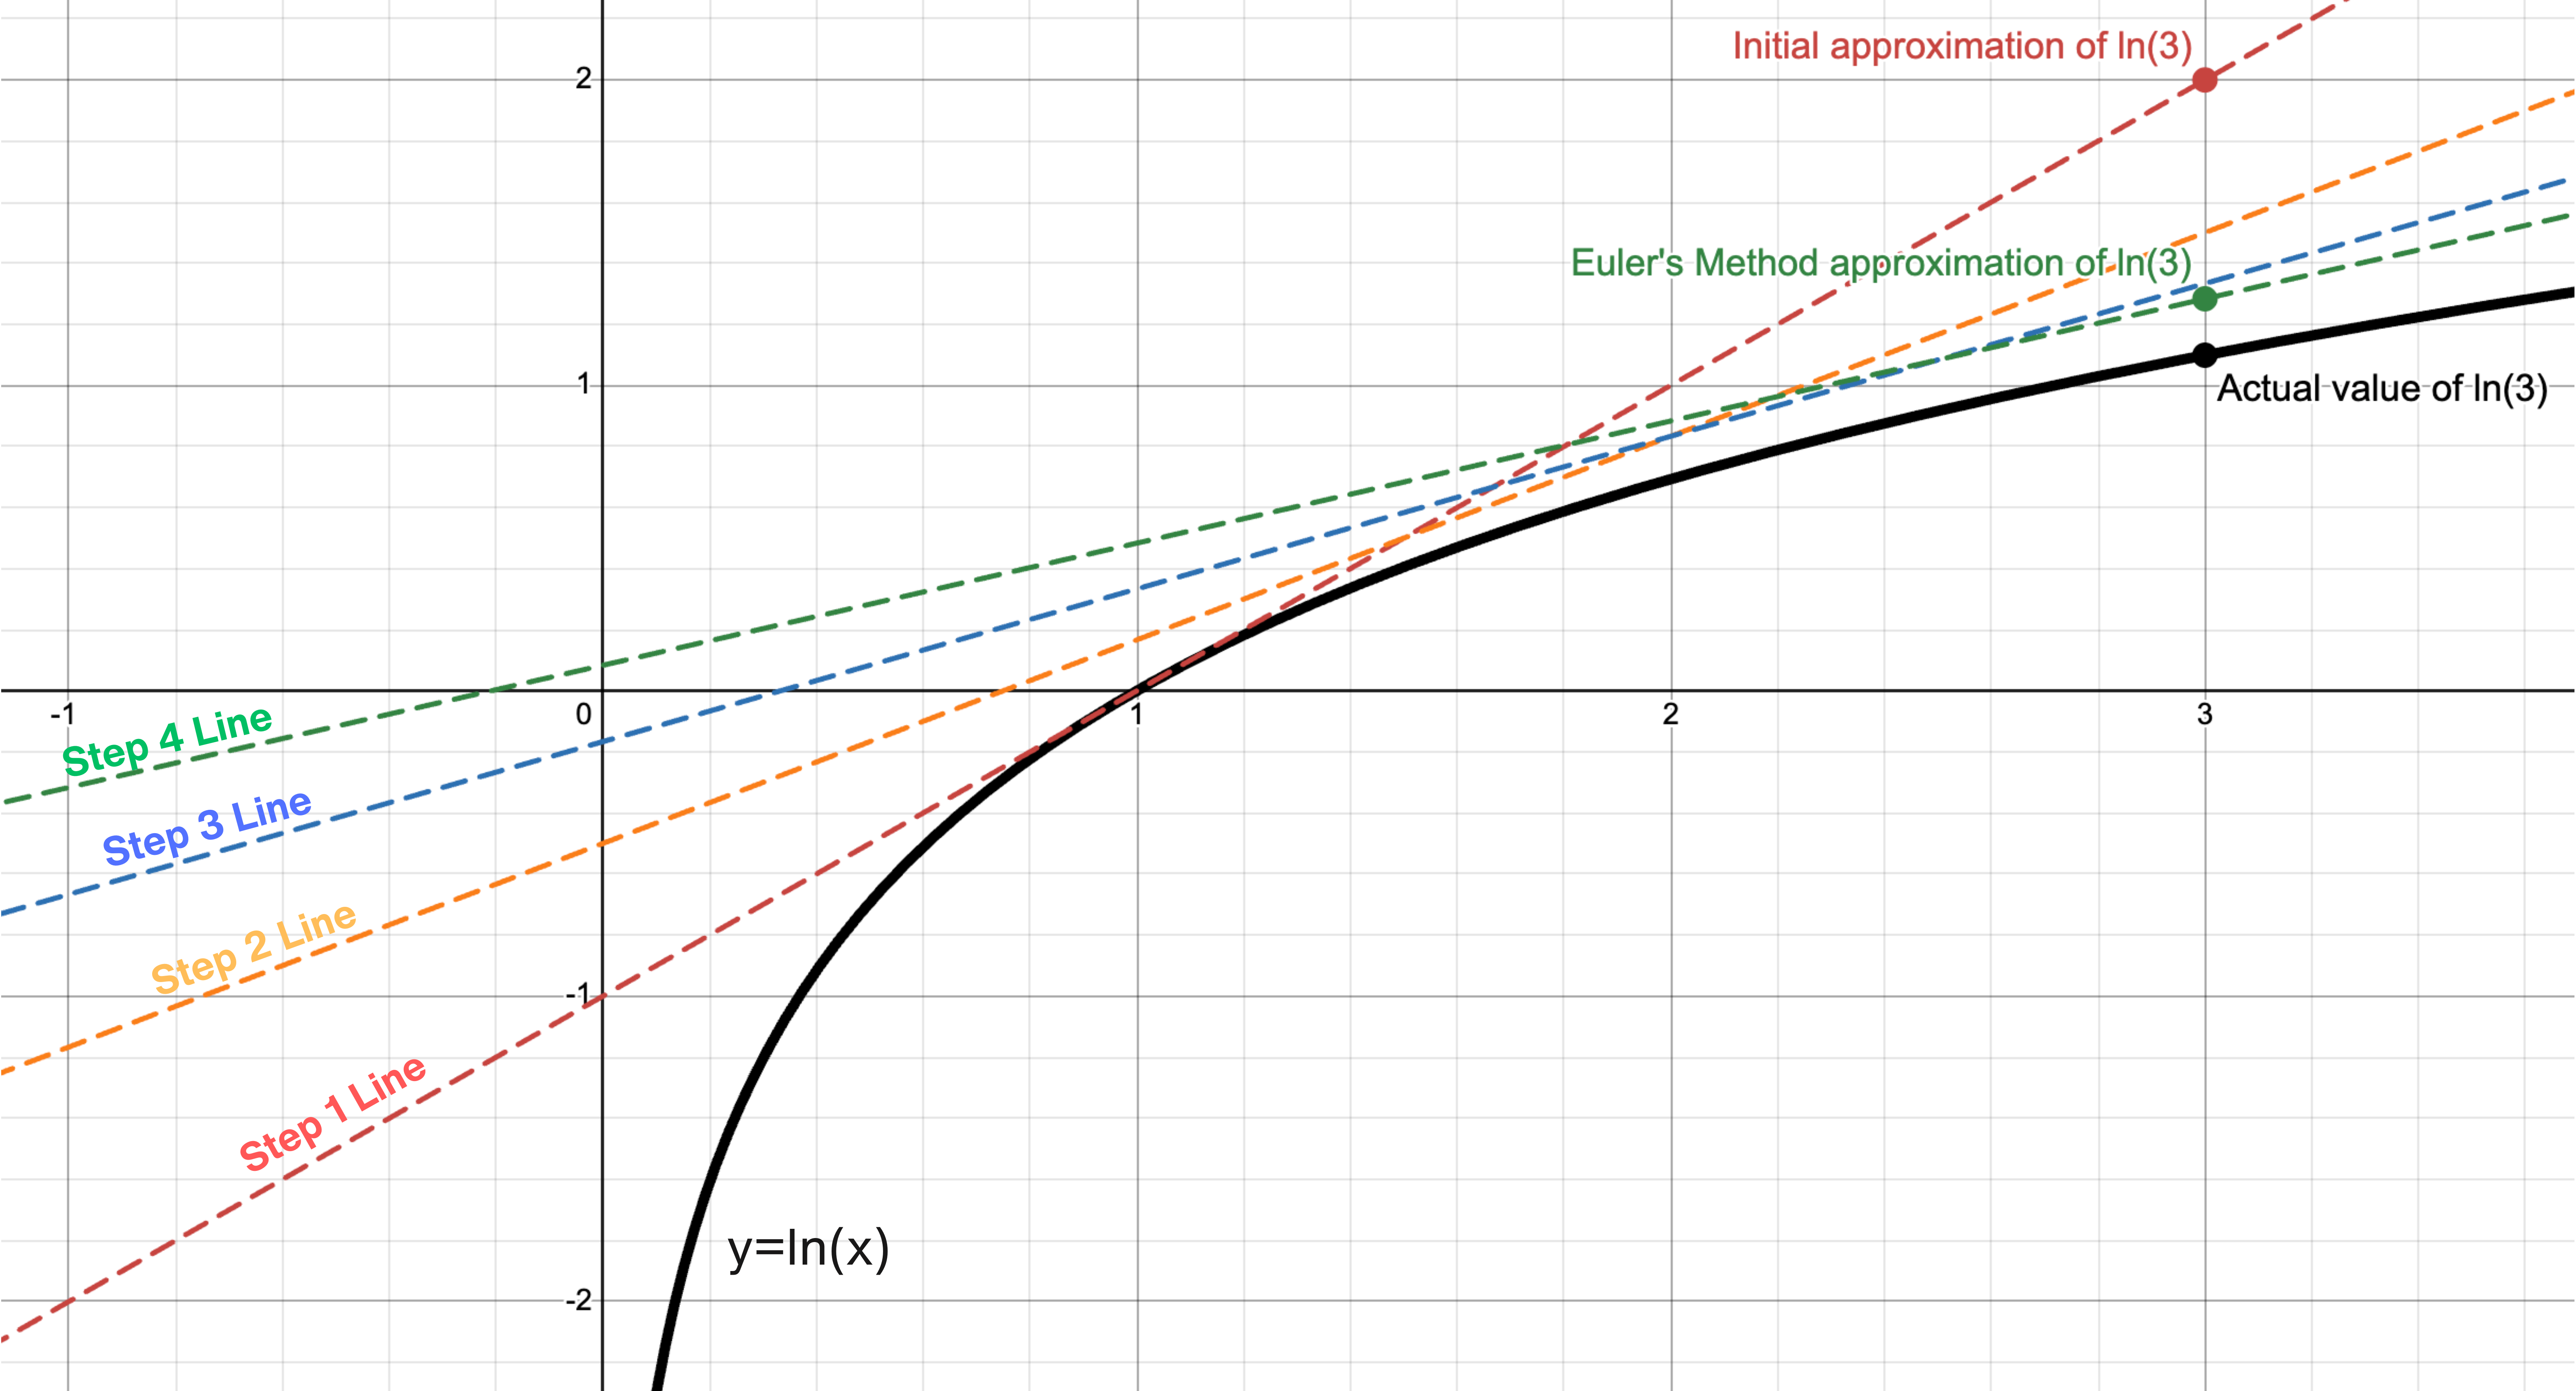
\includegraphics[width=\textwidth]{Support/Chapter 1 Graphics/1.6-Graphic3.png}

We could also use this process to approximate a value for a curve when we only
know its derivative and an initial value on the curve. \par

\begin{tcolorbox}[example]
    \textbf{Ex 1.6.6: } Use Euler's method with a step size of $\dfrac{1}{2}$ to estimate $f\left(\dfrac{5}{2}\right)$ for the function whose derivative is given by $\dfrac{dy}{dx} = 2x + y$ with an initial value of $f(1) = 4$.
\end{tcolorbox}
\begin{tcolorbox}[solution]
    \textbf{Sol 1.6.6: } For this problem, to find the slope for each step, we simply we need to plug in our point into the given differential equation. \begin{align*}
        \def\arraystretch{2.2} 
        \begin{array}{|c|c|c|c|c|c|}
            \hline
            \textbf{Step} & \textbf{Point} & \dfrac{dy}{dx} \textbf{ (Slope)} & \textbf{Tangent Line Equation} & \textbf{New } x & \textbf{New } y \\[5.5pt] \hline
            1 & (1, 4) & 6 & y - 4 = 6(x - 1) & \dfrac{3}{2} & 7 \\[5.5pt] \hline
            2 & \left(\dfrac{3}{2}, 7\right) & 10 & y - 7 = 10\left(x - \dfrac{3}{2}\right) & 2 & 12 \\[5.5pt] \hline
            3 & (2, 12) & 16 & y - 12 = 16(x - 2) & \dfrac{5}{2} & 20 \\[5.5pt]
            \hline
        \end{array}
    \end{align*}
    $f\left(\dfrac{5}{2}\right) \approx y\left(\dfrac{5}{2}\right) = \boxed{20} \forcespace$. We cannot get an exact value for this function, because we have not learned techniques regarding how to solve this differential equation yet.
\end{tcolorbox} \vspace{11pt}

\begin{tcolorbox}[example]
    \textbf{Ex 1.6.7: } Is the approximation in \textbf{Ex 1.6.6} an overestimate or underestimate? Why?
\end{tcolorbox}
\begin{tcolorbox}[solution]
    \textbf{Sol 1.6.7: } To determine this, we need to look at the concavity of the curve -- this requires the second derivative. \begin{align*}
        & \dfrac{dy}{dx} = 2x + y \\[11pt]
        & \dfrac{d^2y}{dx^2} = 2 + \dfrac{dy}{dx} && \text{Don't forget implicit differentiation!} \\[11pt]
        & \dfrac{d^2y}{dx^2} = 2 + (2x + y) \\[11pt]
        & \dfrac{d^2y}{dx^2} \eval_{(1, 4)} = 2 + 2(1) + 4 = 8 && \text{Plug in our initial value}
    \end{align*}
    Since the second derivative is positive, our curve is concave up at this point, which means our tangent line lies under the curve. This is indicative of an $\boxed{\text{underestimate}} \smallforcespace$.
\end{tcolorbox}

Generally: \par

\begin{center}
    \fbox{\fbox{\begin{minipage}{0.96 \textwidth}
        \begin{tabbing}
            $\rightarrow$ \= Your approximation will be an \textbf{overestimate} if the curve is \textbf{concave down} (since \\
            \> your ``tangent lines'' will be above the curve). \\[11pt]
            $\rightarrow$ \= Your approximation will be an \textbf{underestimate} if the curve is \textbf{concave up} (since \\
            \> your ``tangent lines'' will be below the curve).
        \end{tabbing}
    \end{minipage}}}
\end{center}

\begin{tcolorbox}[example]
    \textbf{Ex 1.6.8: } Use Euler's method with four equal step sizes to approximate $f(2)$ for $\dfrac{dy}{dx} = 3y - x$, given $f(0) = 1$. Is this an overestimate or an underestimate?
\end{tcolorbox} 
\begin{tcolorbox}[solution]
    \textbf{Sol 1.6.8: } First, let's figure out our step sizes. We know that we start with $x = 0$, and we need to end up at $x = 2$. Therefore, four equal step sizes means that each step must be $+\dfrac{1}{2} \forcespace$. \par
    Next, let's make our table: \begin{align*}
        \def\arraystretch{2.2} 
        \begin{array}{|c|c|c|c|c|c|}
            \hline
            \textbf{Step} & \textbf{Point} & \dfrac{dy}{dx} \textbf{ (Slope)} & \textbf{Tangent Line Equation} & \textbf{New } x & \textbf{New } y \\[5.5pt] \hline
            1 & (0, 1) & 3 & y - 1 = 3(x - 0) & \dfrac{1}{2} & \dfrac{5}{2} \\[5.5pt] \hline
            2 & \left(\dfrac{1}{2}, \dfrac{5}{2}\right) & 7 & y - \dfrac{5}{2} = 7\left(x - \dfrac{1}{2}\right) & 1 & 6 \\[5.5pt] \hline
            3 & (1, 6) & 17 & y - 6 = 17(x - 1) & \dfrac{3}{2} & \dfrac{29}{2} \\[5.5pt] \hline
            4 & \left(\dfrac{3}{2}, \dfrac{29}{2}\right) & 42 & y - \dfrac{29}{2} = 42\left(x - \dfrac{3}{2}\right) & 2 & \dfrac{71}{2} \\[5.5pt]
            \hline
        \end{array}
    \end{align*}
    We can see that $f(2) \approx y(2) = \boxed{\dfrac{71}{2}} \forcespace$. Now, let's solve for the second derivative to find out if this is an overestimate or underestimate. \begin{align*}
        & \dfrac{d^2y}{dx^2} = 3\dfrac{dy}{dx} - 1 = 9y - 3x - 1 \\[11pt]
        & \dfrac{d^2y}{dx^2} \eval_{(0, 1)} = 9(1) - 3(0) - 1 = 8
    \end{align*}
    Because the positive second derivative indicates that $y$ is concave up at $(0, 1)$, our Euler's Method result is going to be an $\boxed{\text{underestimate}} \smallforcespace$.
\end{tcolorbox}

\newpage

\textbf{\large{1.6 Free Response Homework}} \par

Complete the following: \par

\onequestion{1. Find the equation of the line tangent to $y = x^4 + 2e^x$ at the point $(0, 2)$.} \\[11pt]
\onequestion{2. Find the equation of the line tangent to $y = x + \cos (x)$ at the point $(0, 1$).} \\[11pt]
\onequestion{3. Find the equation of the line tangent to $y = \sec (x) - 2\cos (x)$ at the point $\left(\dfrac{\pi}{3}, 0\right)$.} \\[11pt]
\onequestion{4. Find the equation of the line tangent to $y = x^2e^{-x}$ at the point $\left(1, \dfrac{1}{e}\right)$.} \\[11pt]
\onequestion{5. Find the equation of the line tangent to $y = \dfrac{2}{\pi}x + \cos (4x)$ when $x = \dfrac{\pi}{2}$.} \\[11pt]
\onequestion{6. Find the equation of the line tangent to $y = \dfrac{x^2 - 3}{x^2 - 4}$ when $x = -1$.} \\[11pt]
\onequestion{7. Find the equation of the line tangent to $f(x) = x\sqrt[4]{7 + x^2}$ when $x = 3$.} \\[11pt]
\onequestion{8. Find the equation of the line tangent to $y = e^{x\sin (4x)} + 2$ when $x = 0$.} \\[11pt]
\onequestion{9. Find the equation of the line tangent to $f(x) = x^5 - 5x + 1$ when $x = -2$ and use it to get an approximate value of $f(-1.9)$.} \\[11pt]
\onequestion{10. Find the equation of the line tangent to $f(x) = x\sqrt[3]{1 - x^2}$ when $x= 3$ and use it to get an approximate value of $f(3.1)$.} \\[11pt]
\onequestion{11. Find all points on the graph of $y = 2\sin (x) + \sin^2 (x)$ where the tangent line is horizontal.} \\[11pt]
\onequestion{12. Find all points on the graph of $y = 2x^3 + 3x^2 - 12x + 1$ where the tangent line is horizontal.} \\[11pt]
\onequestion{13. Find the equation of the lines tangent and normal to $y = -\dfrac{2x}{x^2 + 16}$ at $x = -1$.} \\[11pt]
\onequestion{14. Find the equation of the lines tangent and normal to $y = -\dfrac{3x}{x^2 + 1}$ at $x = 1$.} \\[11pt]
\onequestion{15. Find the equation of the lines tangent and normal to $y = \dfrac{x^2 - 4x + 3}{2x^2 - 5x - 3}$ at $x = 2$.} \\[11pt]
\onequestion{16. Find the equation of the lines tangent and normal to $y = x\sin \left(\dfrac{\pi}{2}\ln x\right)$ when $x = e$.} \\[11pt]
\onequestion{17. Find the equation of the lines tangent and normal to $y = x\sin \left(\dfrac{1}{x}\right)$ when $x = \dfrac{4}{\pi}$.} \\[11pt]
\onequestion{18. Use Euler's Method with 2 equal step sizes to find an approximation for $f(0)$, given that $f(-1) = 2$ and $\dfrac{dy}{dx} = 6x^2 - x^2y$.} \\[11pt]
\onequestion{19. Use Euler's Method with 4 equal step sizes to find an approximation for $f(1.4)$, given that $f(1) = 0$ and $f(x) = \ln (2x - 1)$.} \\[11pt]
\onequestion{20. Use Euler's Method with 3 equal step sizes to find an approximation for $f(2.6)$, given that $f(2) = -2$ and $\dfrac{dy}{dx} = 2x + y$.} \\[11pt]

\textbf{\large{1.6 Multiple Choice Homework}} \par

\begin{questions}
    \question Let $f$ be the function given by $f(x) = 2e^{4x^2}$. For what value of $x$ is the slope of the line tangent to the graph of $f$ at $\left(x, f(x)\right)$ equal to $3$? \\

    \begin{oneparchoices}
        \choice $0.168$ 
        \choice $0.274$
        \choice $0.318$
        \choice $0.342$
        \choice $0.551$
    \end{oneparchoices} \par \horizontalline

    \question Which of the following is an equation of the line tangent to the graph of $f(x) = x^6 + x^5 + x^2$ at the point where $f'(x) = -1$? \\

    \begin{oneparchoices}
        \choice $-3x - 2$
        \choice $-3x + 4$
        \choice $-x + 0.905$ \\[11pt]
        \makebox[0.23 \textwidth] \choice $-x + 0.271$
        \makebox[0.27 \textwidth]\choice $-x - 0.271$
    \end{oneparchoices} \par \horizontalline

    \question At what point on the graph of $y = \dfrac{1}{2}x^2$ is the tangent line parallel to the line $2x - 4y = 3$? \\

    \begin{oneparchoices}
        \choice $\left(\dfrac{1}{2}, -\dfrac{1}{2}\right)$
        \choice $\left(\dfrac{1}{2}, -\dfrac{1}{8}\right)$
        \choice $\left(\dfrac{1}{2}, -\dfrac{1}{4}\right)$
        \choice $\left(1, -\dfrac{1}{2}\right)$
        \choice $(2, 2)$
    \end{oneparchoices} \par \horizontalline

    \question A normal line to the graph of a function $f$ at the point $(x, f(x))$ is defined to be the line perpendicular to the tangent line at that point. An equation of the normal line to the curve $y = \sqrt[3]{x^2 - 1}$ at the point where $x = 3$ is \\

    \begin{oneparchoices}
        \choice $y + 12x = 38$
        \choice $y - 4x = 10$
        \choice $y + 2x = 4$ \\[11pt]
        \makebox[0.25 \textwidth] \choice $y + 2x = 8$
        \makebox[0.27 \textwidth] \choice $y - 2x = -4$
    \end{oneparchoices} \par \horizontalline

    \question Let $y = f(x)$ be the solution to the differential equation $\dfrac{dy}{dx} = \dfrac{4x}{y} \forcespace$ with the initial condition $f(0) = 1$. What is the best approximation for $f(1)$ using Euler's Method, starting at $x = 0$ with a step size of $0.5$? \\

    \begin{oneparchoices}
        \choice $1$
        \choice $2$
        \choice $\sqrt{5}$
        \choice $2.5$
        \choice $3$
    \end{oneparchoices} \par \horizontalline

    \question Let $y = f(x)$ be the solution to the differential equation $\dfrac{dy}{dx} = x - y^2 \forcespace$ with the initial condition $f(0) = 1$. What is the best approximation for $f(2)$ using Euler's Method, starting at $x = 0$ with a step size of $1$? \\

    \begin{oneparchoices}
        \choice $-1$
        \choice $0$
        \choice $1$
        \choice $2$
        \choice $3$
    \end{oneparchoices} \par \horizontalline

    \question Let $y = f(x)$ be the solution to the differential equation $\dfrac{dy}{dx} = y - x \forcespace$ with the initial condition $f(1) = 2$. What is the best approximation for $f(2)$ using Euler's Method, starting at $x = 1$ with a step size of $0.5$? \\

    \begin{oneparchoices}
        \choice $1$
        \choice $2$
        \choice $3$
        \choice $4.5$
        \choice $6$
    \end{oneparchoices} \par \horizontalline

    \question The graph of $y = f'(x)$ is given below. Use this information and the fact that $f(0) = 3$ to find an approximate value of $f(1)$ using Euler's method with 2 equal step sizes. \\

    \begin{center}
        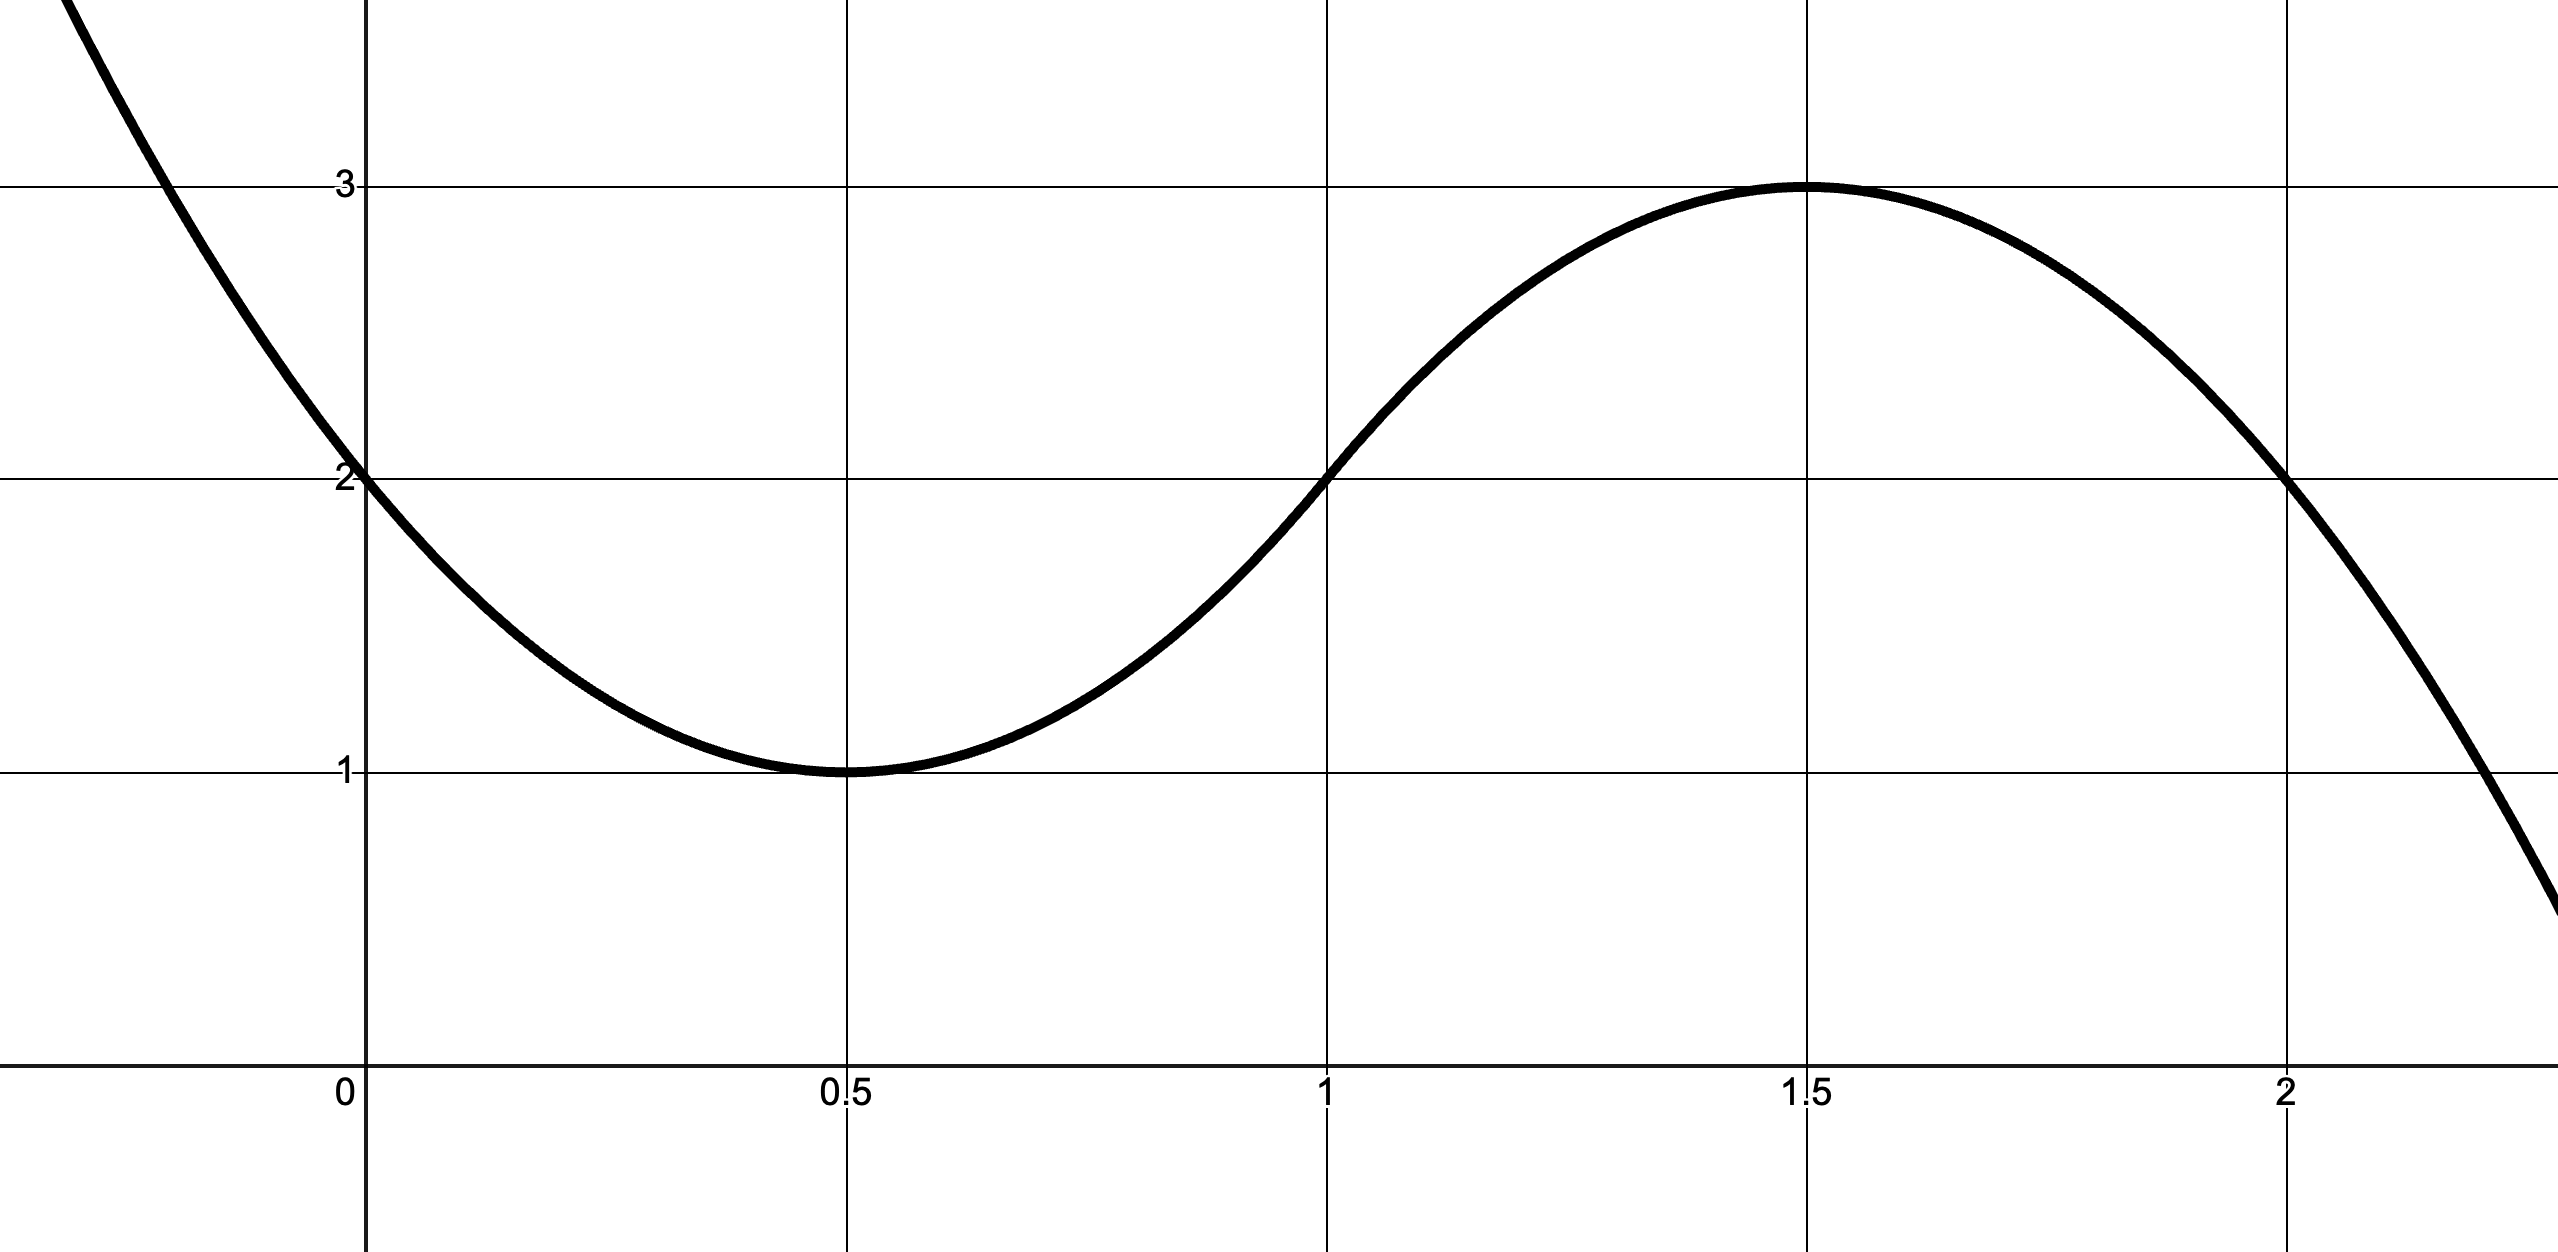
\includegraphics[width = 0.6\textwidth]{Support/Chapter 1 Graphics/1.6-Graphic4.png}
    \end{center} 

    \begin{oneparchoices}
        \choice $2.5$
        \choice $3.5$
        \choice $4$
        \choice $4.5$
        \choice $5$
    \end{oneparchoices} \par \horizontalline

    \question The table below gives selected values for the derivative of a function $g$ on the interval $-1 \leq x \leq 2$. If $g(-1) = -2$ and Euler's Method with a step size of $1.5$ is used to approximate $g(2)$, what is the resulting approximation? \begin{align*}
        \arraycolsep=11pt\def\arraystretch{1.5}
        \begin{array}{|c|c|c|c|c|c|c|c|}
            \hline
            x & -1.0 & -0.5 & 0 & 0.5 & 1.0 & 1.5 & 2.0 \\ \hline
            f'(x) & 2 & 4 & 3 & 1 & 0 & -3 & -6 \\
            \hline
        \end{array}
    \end{align*}

    \begin{oneparchoices}
        \choice $-6.5$
        \choice $-1.5$
        \choice $1.5$
        \choice $2.5$
        \choice $3$
    \end{oneparchoices} \par \horizontalline

    \question The equation of the line \textbf{normal} to the graph of $y = \dfrac{3x + 4}{4x - 3}$ at $(1, 7)$ is \\

    \begin{oneparchoices}
        \choice $25x + y = 32$ 
        \choice $25x - y = 18$
        \choice $7x - y = 0$ \\[11pt]
        \makebox[0.23\textwidth] \choice $x - 25y = -174$ 
        \makebox[0.23\textwidth] \choice $x + 25y = 176$
    \end{oneparchoices} \par \horizontalline

    \question The equation of the line \textbf{normal} to the graph of $y = 3x\sqrt{x^2 + 6} - 3$ at $(0, -3)$ is \\

    \begin{oneparchoices}
        \choice $3\sqrt{6}x + y = -3$
        \choice $3\sqrt{6}x - y = -3$
        \choice $x + 3\sqrt{6}y = -3$ \\[11pt]
        \makebox[0.2\textwidth] \choice $x - 3\sqrt{6}y = 9\sqrt{6}$
        \makebox[0.23\textwidth] \choice $x + 3\sqrt{6}y = -9\sqrt{6}$
    \end{oneparchoices} \par \horizontalline
\end{questions}